\documentclass[10pt,a4paper]{article}
\usepackage{homework} % See homework.sty %
\usepackage{graphicx}
\usepackage{float}
\usepackage{array}
\usepackage[export]{adjustbox}  
\newcolumntype{M}[1]{>{\centering\arraybackslash}m{#1}}

\author{1155193237 - Yu Ching Hei\\email: chyu2@cse.cuhk.edu.hk}
\title{CENG3420 - Computer Organization \& Design\\Lab1 Report}
\pagestyle{fancy}
\renewcommand{\headrulewidth}{0pt}
\fancyhf{}
\cfoot{\thepage}
\date{Date: \today}
\begin{document}
\maketitle

\question{
	\label{Question1}
    Write a RISC-V assembly program step by step as shown below:
    \begin{enumerate}
        \item Define three variables var1, var2 and var3 which will be loaded from terminal using syscall.
        \item Increase var1 by 3, multiply var2 by 2.
        \item increase var3 by var1 + var2.
        \item print var1, var2 and var3 to terminal using syscall.
    \end{enumerate}
}

\begin{ans} 

    First, I declared a variable of datatype “.ascii” and named it as endl, which stored the constant 
string literal `\textbackslash n'. 

    Then the program will require the user to input 3 integers by loading immediate 5 to change the system call 
mode into readInt mode. Then issue a system call to request for input. After the system call, the integer would 
be stored at a0 as return value. Then I perform the data copy from a0 to t0 by mv a0, t0 and the same for t1 
and t2 as well. Then I perform the arithmetic to the data. By running addi t0, t0, 3, I can add a hard code 
constant 3 to t0, then store back to t0 (t0 = t0 + 3). 
 
    Since mul instruction does not accept immediate, so I loaded a register t3 with the multiplier “2” using the li t3, 2. 
 
    Then I perform the multiplication by multiplying t1 with t3 and then stored back to t3 (t1 = t1 * t3) by doing mul t1, t1, t3. 
Followed by the last modification to the numbers, since we cannot sum a value with 2 other value at the same time, to perform 
var3 = var3 + var1 + var2, I have to do the addition twice. 
 
	First I added t0 to t2 then stored it back to t2, then I add another t1 to t2 and then store it back to t2. For a cleaner code, 
I wrote a function for printing prtNL for printing a new line character after printing each variable. 
 
	In the prtNL function, I first changed the mode of system call to 4 which is printString from address. 
Then I load the address from memory by la a0, endl. Then I issue a system call and return to the return address. 
 
	Now I start to print the variable to the console one by one. I change the system call mode to 1 which is printInt, 
then copy the data from the registers that store the data representing var1, var2 and var3 respectively 
to the a0 register which is the function argument register. 
 
	Finally, I loaded register a7 with 10, which changes the system call mode to exit the program with code 0. 
 
\break

\begin{table}[htbp]
    \begin{center}
        \caption{Main Code for Question 1}
        \begin{tabular}{|M{2.5cm}|M{3.5cm}|M{2cm}|M{4cm}|}
            \hline
            Input Integer & Add and Multiply & Print Integer \& Exit & New Line Function\\
            \hline
            \centering
            % 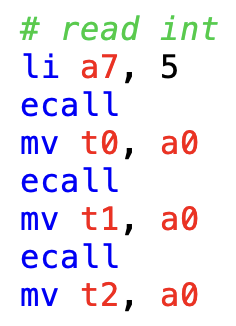
\includegraphics[scale = 0.5]{Lab1-1-1.png} &
            % 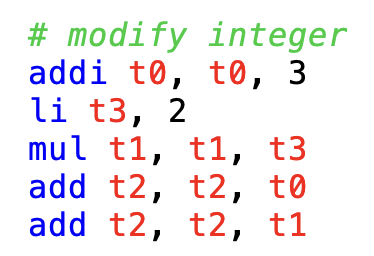
\includegraphics[scale = 0.5]{Lab1-1-2.png} &
            % 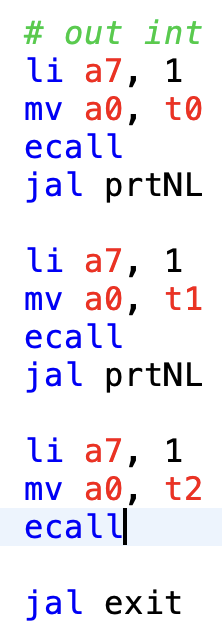
\includegraphics[scale = 0.5]{Lab1-1-3.png} &
            % 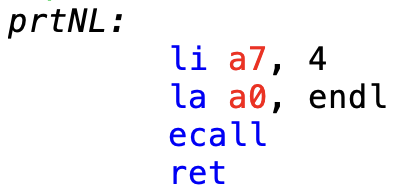
\includegraphics[scale = 0.5]{Lab1-1-4.png} \\
        
    \end{tabular}
    \end{center}
\end{table}

\begin{figure}[H]
    \caption{Console Results}
    % 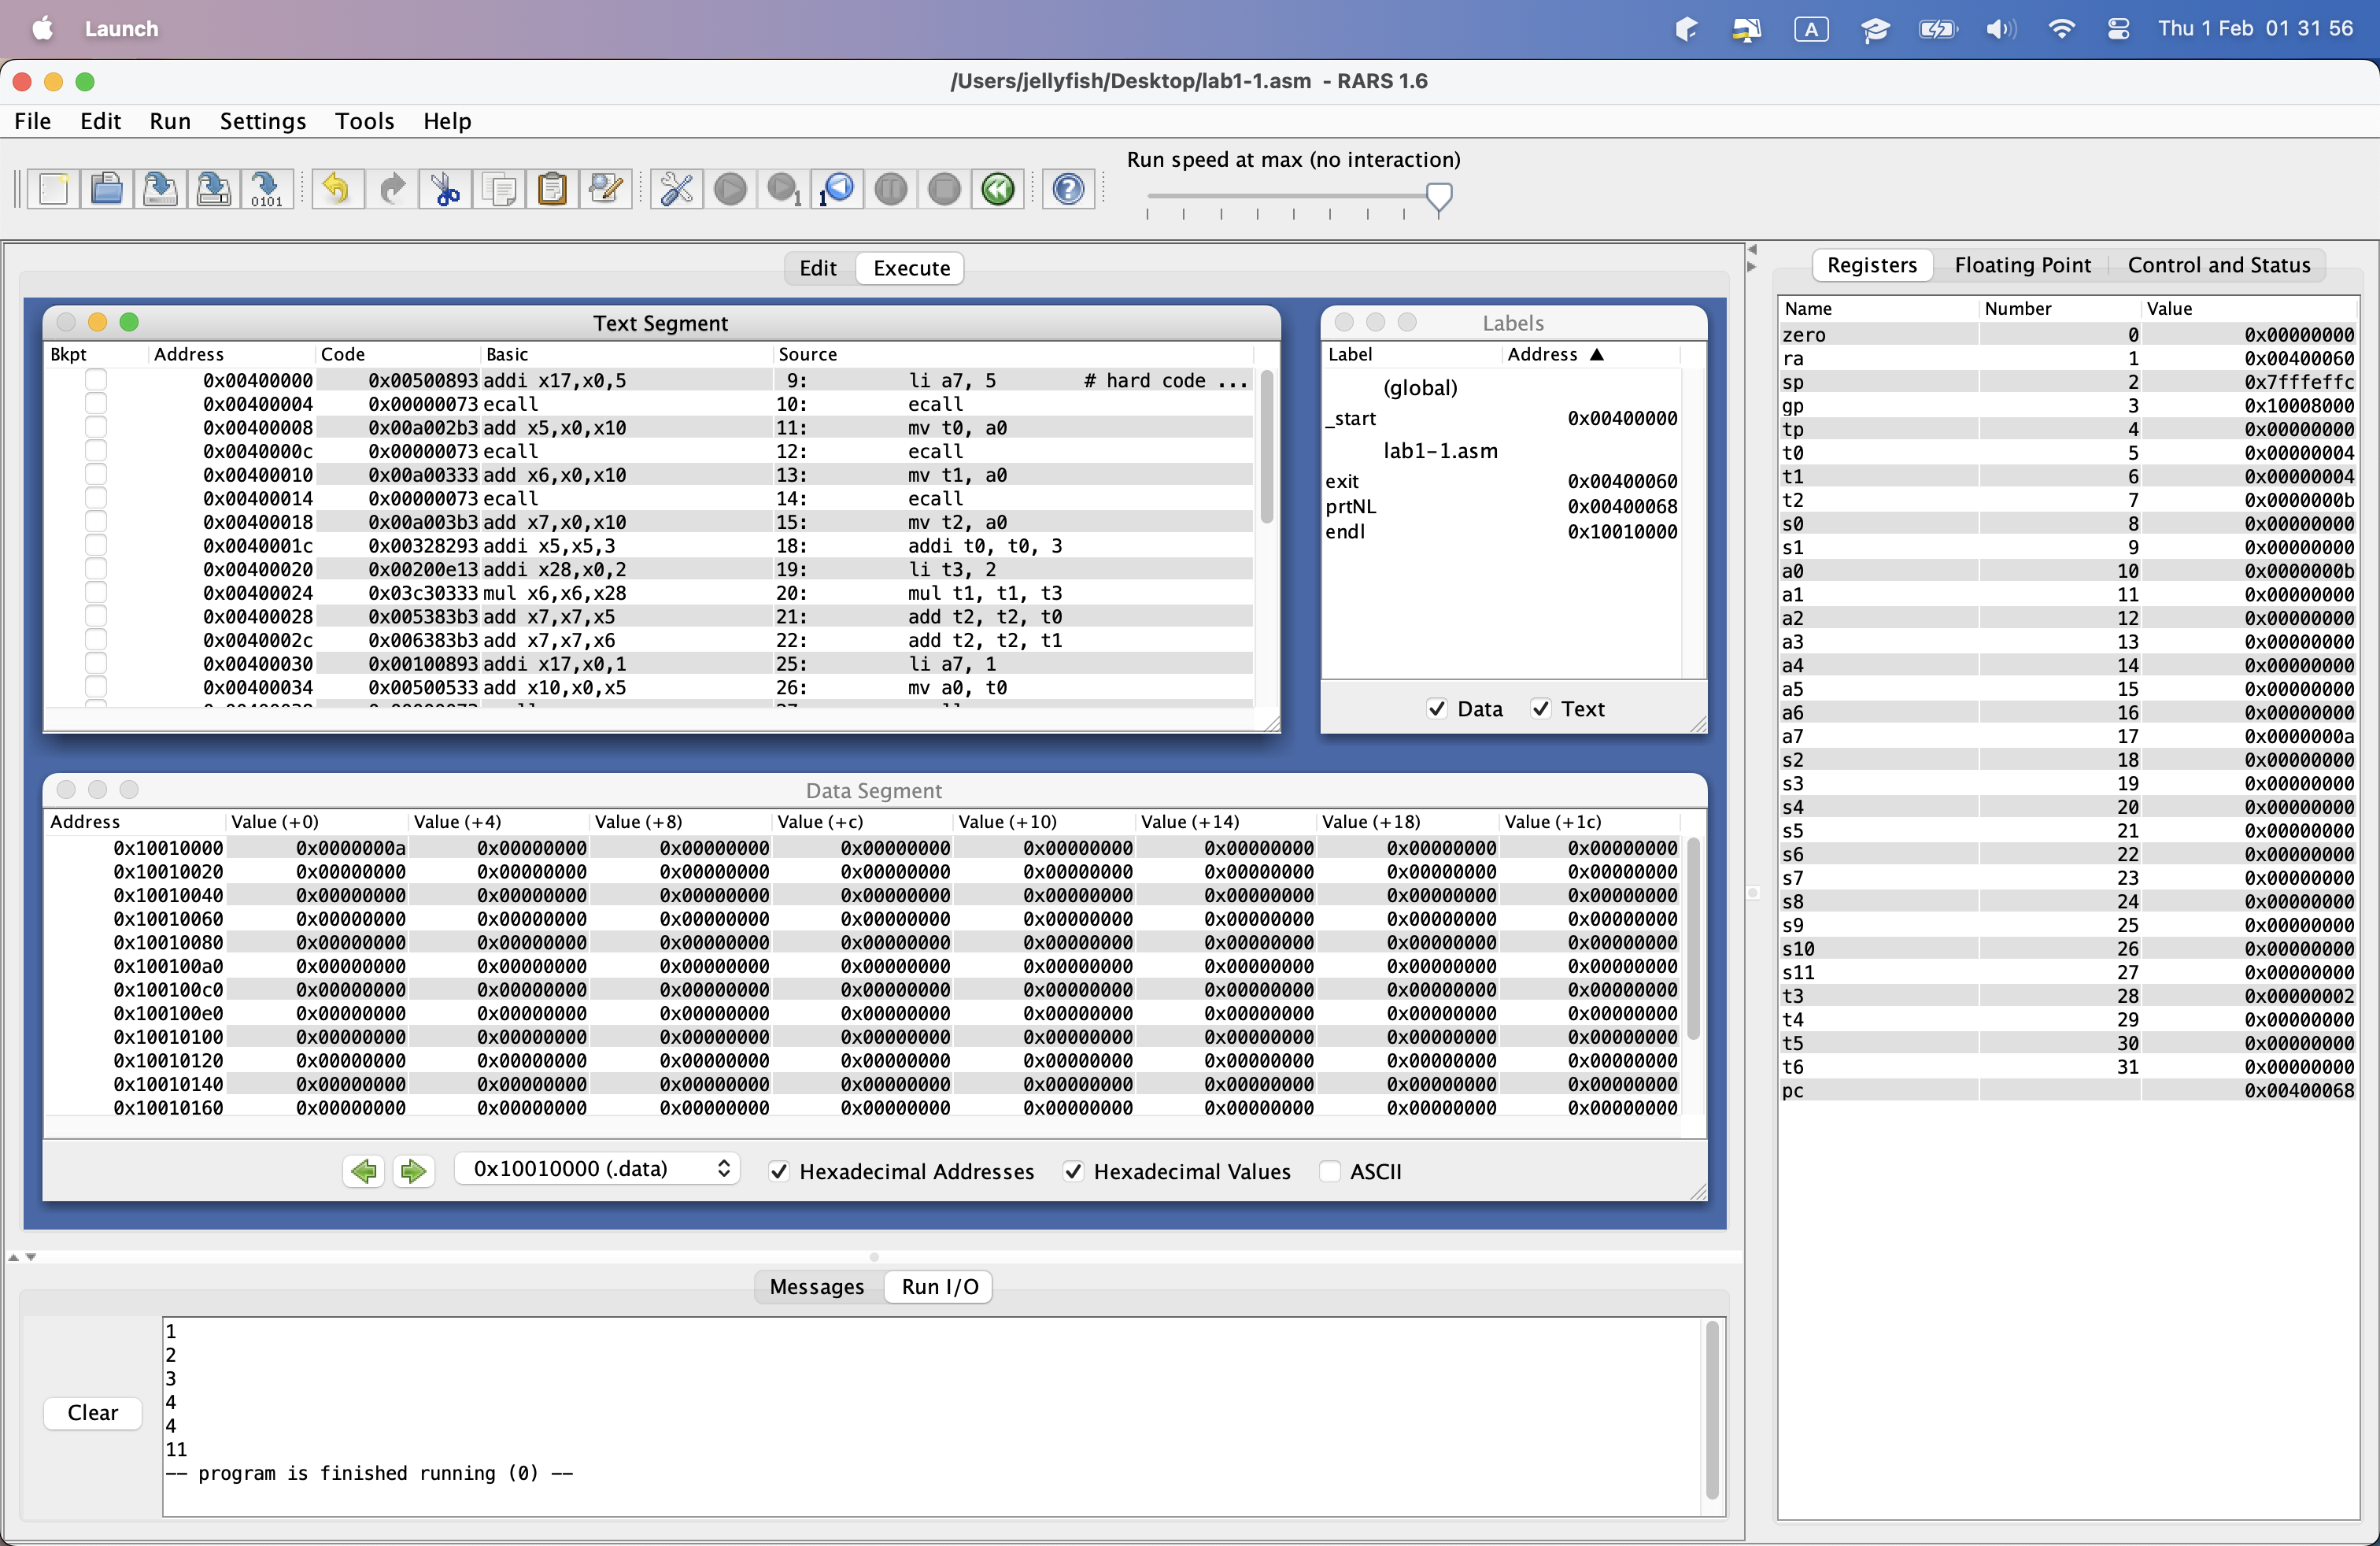
\includegraphics[width=1\linewidth]{Lab1-1-5.png}
\end{figure}
 
\end{ans}

\end{document}